\chapter[ANTLR]{ANTLR --- \emph{Another Tool for Language Recognition}}
Es gibt eine Reihe von Werkzeugen, die in der Lage sind, einen Top-Down-Parser automatisch
zu erzeugen.  Das Werkzeug, das in meinen Augen am besten ausgereift ist, ist
\textsc{Antlr} \cite{parr:2012,parr:2013}.  Der Name steht f\"ur 
\emph{\underline{an}other \underline{t}ool for \underline{l}anguage \underline{r}ecognition}\footnote{
Der Name \textsc{Antlr} kann au{\ss}erdem auch als Abk\"urzung f\"ur \underline{ant}i \underline{LR} verstanden
werden. Hier steht ``LR'' f\"ur \emph{LR-Parser}.  Dies ist eine Klasse von Parsern, die nicht \emph{top-down} 
sondern stattdessen \emph{bottom-up} arbeiten.  Wir werden diese Klasse von Parsern sp\"ater noch ausf\"uhrlich 
diskutieren.
}.
Sie finden dieses Werkzeug im Internet unter der folgenden Adresse 
\\[0.2cm]
\hspace*{1.3cm}
\href{http://www.antlr.org}{\texttt{http://www.antlr.org}}.
\\[0.2cm]
In dieser Vorlesung werden wir die Version 4.5.1 verwenden.  Das Werkzeug \textsc{Antlr} ist in der
Lage, Parser in den Sprachen \textsl{Java}, \texttt{C\#} und \textsl{Python} zu erzeugen.

Zun\"achst f\"uhren wir \textsc{Antlr} anhand verschiedener Beispiele ein, durch die wir die 
wichtigsten Eigenschaften des Werkzeugs demonstrieren k\"onnen.  In sp\"ateren Kapiteln werden wir
die Theorie von Top-Down-Parsern untersuchen.
\textsc{Antlr} unterst\"utzt die Verwendung von \textsc{Ebnf}-Grammatiken.  


\section{Ein Parser f\"ur arithmetische Ausdr\"ucke}
Wir beginnen mit einem Parser f\"ur arithmetische Ausdr\"ucke, die entsprechend der in
Abbildung \ref{fig:Expr} auf Seite \pageref{fig:Expr} gezeigten Grammatik aufgebaut sind.
Diese Grammatik l\"asst sich nun mit Hilfe von \textsc{Antlr} wie in Abbildung
\ref{fig:Expr.g4} gezeigt implementieren.  Wir diskutieren diese Umsetzung Zeile f\"ur Zeile.

\begin{figure}[!ht]
\centering
\begin{Verbatim}[ frame         = lines, 
                  framesep      = 0.3cm, 
                  labelposition = bottomline,
                  numbers       = left,
                  numbersep     = -0.2cm,
                  xleftmargin   = 0.8cm,
                  xrightmargin  = 0.8cm,
                ]
    grammar Expr;
    
    start   : expr
            ;
    
    expr    : expr ('+'|'-') product 
            | product        
            ;
    
    product : product ('*'|'/') factor 
            | factor
            ;
    
    factor  : '(' expr ')'
            | NUMBER
            ;
    
    NUMBER  : '0'|[1-9][0-9]*;
    WS      : [ \v\t\n\r] -> skip;
\end{Verbatim}
\vspace*{-0.3cm}
\caption{\textsc{Antlr}-Spezifikation eines Parsers f\"ur arithmetische Ausdr\"ucke.}
\label{fig:Expr.g4}
\end{figure}


\begin{enumerate}
\item In Zeile 1 spezifizieren wir mit dem Schl\"usselwort \texttt{grammar} den Namen der Grammatik.
      In unserem Fall hat die Grammatik also den Namen \texttt{Expr}.  Der Name  der Datei, in der
      die Grammatik abgespeichert ist, wird aus dem Namen der Grammatik durch Anh\"angen der Endung ``\texttt{.g4}''
      gebildet, daher muss die gezeigte Grammatik in einer Datei mit dem Namen ``\texttt{Expr.g4}''
      abgespeichert werden.      
\item Zeile 3 enth\"alt die Grammatik-Regel f\"ur die syntaktische Variable
      \textsl{start}.  Die dort gezeigte Grammatik-Regel entspricht mathematisch der Regel
      \\[0.2cm]
      \hspace*{1.3cm}
      $\textsl{start} \rightarrow \textsl{expr}$.
      \\[0.2cm]
      Beachten Sie, dass linke und rechte Seite einer Grammatik-Regel durch einen Doppelpunkt
      getrennt werden.
      Jede Grammatik-Regel wird durch ein Semikolon ``\texttt{;}'' beendet.
\item Zeile 6 enth\"alt die Grammatik-Regel f\"ur die syntaktische Variable
      \textsl{expr}.  Zu beachten ist hier, dass die Terminale ``\texttt{+}'' und
      ``\texttt{-}'' bei \textsc{Antlr} in einfache Anf\"uhrungszeichen gesetzt werden
      m\"ussen.  Zus\"atzlich sehen wir, dass die
      verschiedenen Grammatikregeln, welche dieselbe syntaktische
      Variable definieren, durch das Zeichen ``\texttt{|}'' von einander getrennt werden.
\item Entsprechend enthalten die Zeilen 10 und 14 die Grammatik-Regeln f\"ur die syntaktischen
      Variablen \textsl{product} und \textsl{factor}.  

\item Bei \textsc{Antlr} werden die grammatikalische Struktur und die lexikalische
      Struktur der Eingabe in derselben Datei definiert.  Um syntaktische Variablen und
      Terminale von einander unterscheiden zu k\"onnen, wird vereinbart, dass Terminale mit
      einem Gro{\ss}buchstaben beginnen,\footnote
      {Es ist Konvention, aber nicht vorgeschrieben, dass die 
      Namen von Terminalen nur aus Gro{\ss}buchstaben bestehen.}
      w\"ahrend syntaktische Variablen immer mit einem kleinen
      Buchstaben beginnen.  
      Daher wissen wir, dass der String ``\texttt{NUMBER}'' in Zeile 8
      ein Terminal bezeichnet.
\item In Zeile 18 wird die lexikalische Struktur der mit \texttt{NUMBER} bezeichneten
      Terminale durch einen regul\"aren Ausdruck definiert.  Der regul\"are Ausdruck
      \\[0.2cm]
      \hspace*{1.3cm}
      \texttt{'0'|[1-9][0-9]*;}
      \\[0.2cm]
      steht hier f\"ur eine Folge aus Ziffern.  Diese Folge von Ziffern kann nur dann mit der Ziffer
      ``\texttt{0}'' beginnen, wenn auf die ``\texttt{0}'' keine weitere Ziffer mehr folgt.

      Notice that we have to enclose the first occurrence of ``\texttt{0}'' in single quotes.
      On the other hand, we must not put the digits occurring in the square brackets ``\texttt{[}'' 
      and ``\texttt{]}'' in quotes, since these occur inside a range and characters inside a range
      must never be quoted.
\item Zeile 19 definiert schlie{\ss}lich das Token \texttt{WS}, wobei der Name als Abk\"urzung
      f\"ur \emph{white space} zu verstehen ist.  Hier werden Leerzeichen, Tabulatoren,
      Zeilenumbr\"uche und Wagenr\"uckl\"aufe erkannt.  Nach der lexikalischen Spezifikation
      von \texttt{WS} folgt nach dem Operator ``\texttt{->}'' noch eine semantische Aktion.
      Die spezielle Aktion ``\texttt{skip}'', die hier ausgef\"uhrt wird, wirft das erkannte
      Token einfach weg, ohne es an den Parser weiterzureichen.  Aus diesem Grunde wird das Token
      \texttt{WS} in den Grammatik-Regeln nicht verwendet, denn der Scanner reicht dieses Token nie
      an den Parser weiter.  Insgesamt hat die Regel in Zeile 19 daher den Effekt, Leerzeichen, Tabulatoren,
      Zeilenumbr\"uche und Wagenr\"uckl\"aufe aus der Eingabe zu entfernen.

      In most programming languages, white space has no purpose other than that of separating
      tokens.  Therefore, most \textsc{Antlr} parsers will have a scanner rule that is similar to
      the rule shown in line 19. 
\end{enumerate}
Zusammenfassend enthalten die Zeilen 3 -- 16 also die Definition der grammatikalischen
Struktur, w\"ahrend die Zeilen 18 und 19 die lexikalische Struktur definieren.

Um aus der in Abbildung \ref{fig:Expr.g4} gezeigten Grammatik einen Parser erzeugen zu
k\"onnen,  \"ubersetzen wir diese Datei mit dem folgenden Befehl:
\\[0.2cm]
\hspace*{1.3cm}
\texttt{java -jar /usr/local/lib/antlr-4.4-complete.jar Expr.g4}
\\[0.2cm]
Das setzt nat\"urlich voraus, dass die angegebene Datei \texttt{antlr-4.4-complete.jar} auch
tats\"achlich in dem Verzeichnis \texttt{/usr/local/lib/} zu finden ist.
\textsc{Antlr} erzeugt die folgenden Dateien:
\begin{enumerate}
\item \texttt{ExprParser.java}

      Hier handelt es sich um den eigentlichen Parser.
\item \texttt{ExprLexer.java}

      Hier ist der Scanner implementiert.
\item Zus\"atzlich werden noch die Dateien \texttt{ExprListener.java},
      \texttt{ExprBaseListener.java}, \texttt{Expr.tokens} sowie \texttt{ExprLexer.tokens} erzeugt,
      auf die wir aber nicht weiter eingehen.
\end{enumerate}
Um den erzeugten Parser aufrufen zu k\"onnen, ben\"otigen wir noch ein Treiber-Programm.
Abbildung \ref{fig:ParseExpr.java} zeigt ein solches Programm.

\begin{figure}[!ht]
\centering
\begin{Verbatim}[ frame         = lines, 
                  framesep      = 0.3cm, 
                  labelposition = bottomline,
                  numbers       = left,
                  numbersep     = -0.2cm,
                  xleftmargin   = 0.8cm,
                  xrightmargin  = 0.8cm,
                ]
    import org.antlr.v4.runtime.*;
    import org.antlr.v4.runtime.tree.*;
    
    public class ParseExpr {
    
        public static void main(String[] args) throws Exception {
            ANTLRInputStream  input  = new ANTLRInputStream(System.in);
            ExprLexer         lexer  = new ExprLexer(input);
            CommonTokenStream ts     = new CommonTokenStream(lexer);
            ExprParser        parser = new ExprParser(ts);
            ParseTree         tree   = parser.start();
            System.out.println(tree.toStringTree(parser)); 
        }
    }
\end{Verbatim}
\vspace*{-0.3cm}
\caption{Treiber-Programm f\"ur den von \textsc{Antlr} erzeugten Parser.}
\label{fig:ParseExpr.java}
\end{figure}

\begin{enumerate}
\item In den Zeilen 1 und 2 importieren wir die \textsc{Antlr}-Runtime-Pakete.
      Dort sind u.a.~die Klassen  
      \\[0.2cm]
      \hspace*{1.3cm}
      \texttt{ANTLRInputStream} \quad und \quad \texttt{CommonTokenStream}, 
      \\[0.2cm]
      auf deren Verwendung wir angewiesen sind, definiert.
\item In Zeile 7 wandeln wir die Standard-Eingabe in einen \texttt{ANTLRInputStream} um,
      der dann in Zeile 8 dazu benutzt werden kann, einen Scanner zu erzeugen. 
\item Mit Hilfe des  Scanners erzeugen wir in Zeile 9 einen TokenStream und aus diesem k\"onnen wir 
      in Zeile 10 einen Parser erzeugen.
\item Der Aufruf des Parsers erfolgt in Zeile 11, indem wir den Namen der syntaktischen Variable,
      die wir parsen m\"ochten, als Methode verwenden.
\item Schlie{\ss}lich geben wir den erzeugten Baum noch als Text aus.
\end{enumerate}
\"Ubersetzen wir dieses Programm, so k\"onnen wir den Parser durch den Befehl
\\[0.2cm]
\hspace*{1.3cm}
\texttt{echo  \symbol{34}1 + 2 * 3 - 4\symbol{34} | java -cp /usr/local/lib/antlr-4.4-complete.jar ParseExpr}
\\[0.2cm]
testen.  Wir erhalten die Ausgabe
\\[0.2cm]
\hspace*{0.3cm}
\texttt{(start (expr (expr (product (factor 1))) + (product (product (factor 2)) * (factor 3))))}.
\\[0.2cm]
Geben wir stattdessen den Befehl
\\[0.2cm]
\hspace*{1.3cm}
\texttt{echo \symbol{34}1 + 2 * 3 - 4\symbol{34} | java org.antlr.v4.runtime.misc.TestRig Expr start -gui}
\\[0.2cm]
ein, so erhalten wir, vorausgesetzt dass die Variable \texttt{CLASSPATH} richtig gesetzt ist,
den in Abbildung \ref{fig:expr.eps} gezeigten Syntax-Baum.  Falls wir den Alias \texttt{grun} in der
Datei ``\texttt{.bashrc}'' als
\\[0.2cm]
\hspace*{1.3cm}
\texttt{alias grun='java org.antlr.v4.runtime.misc.TestRig'}
\\[0.2cm]
definiert haben, so k\"onnen wir den Syntax-Baum auch einfacher mit Hilfe des Befehls
\\[0.2cm]
\hspace*{1.3cm}
\texttt{echo \symbol{34}1 + 2 * 3 - 4\symbol{34} | grun Expr start -gui}
\\[0.2cm]
anzeigen lassen.  Zum Aufruf von \textsc{Antlr} bietet sich der Alias
\\[0.2cm]
\hspace*{1.3cm}
\texttt{alias antlr4='java -jar /usr/local/lib/antlr-4.4-complete.jar'}
\\[0.2cm]
an, denn damit k\"onnen wir \textsc{Antlr}  dann \"uber den Befehl
\\[0.2cm]
\hspace*{1.3cm}
\texttt{antlr4 Expr.g4}
\\[0.2cm]
aufrufen.

\begin{figure}[!ht]
  \centering
      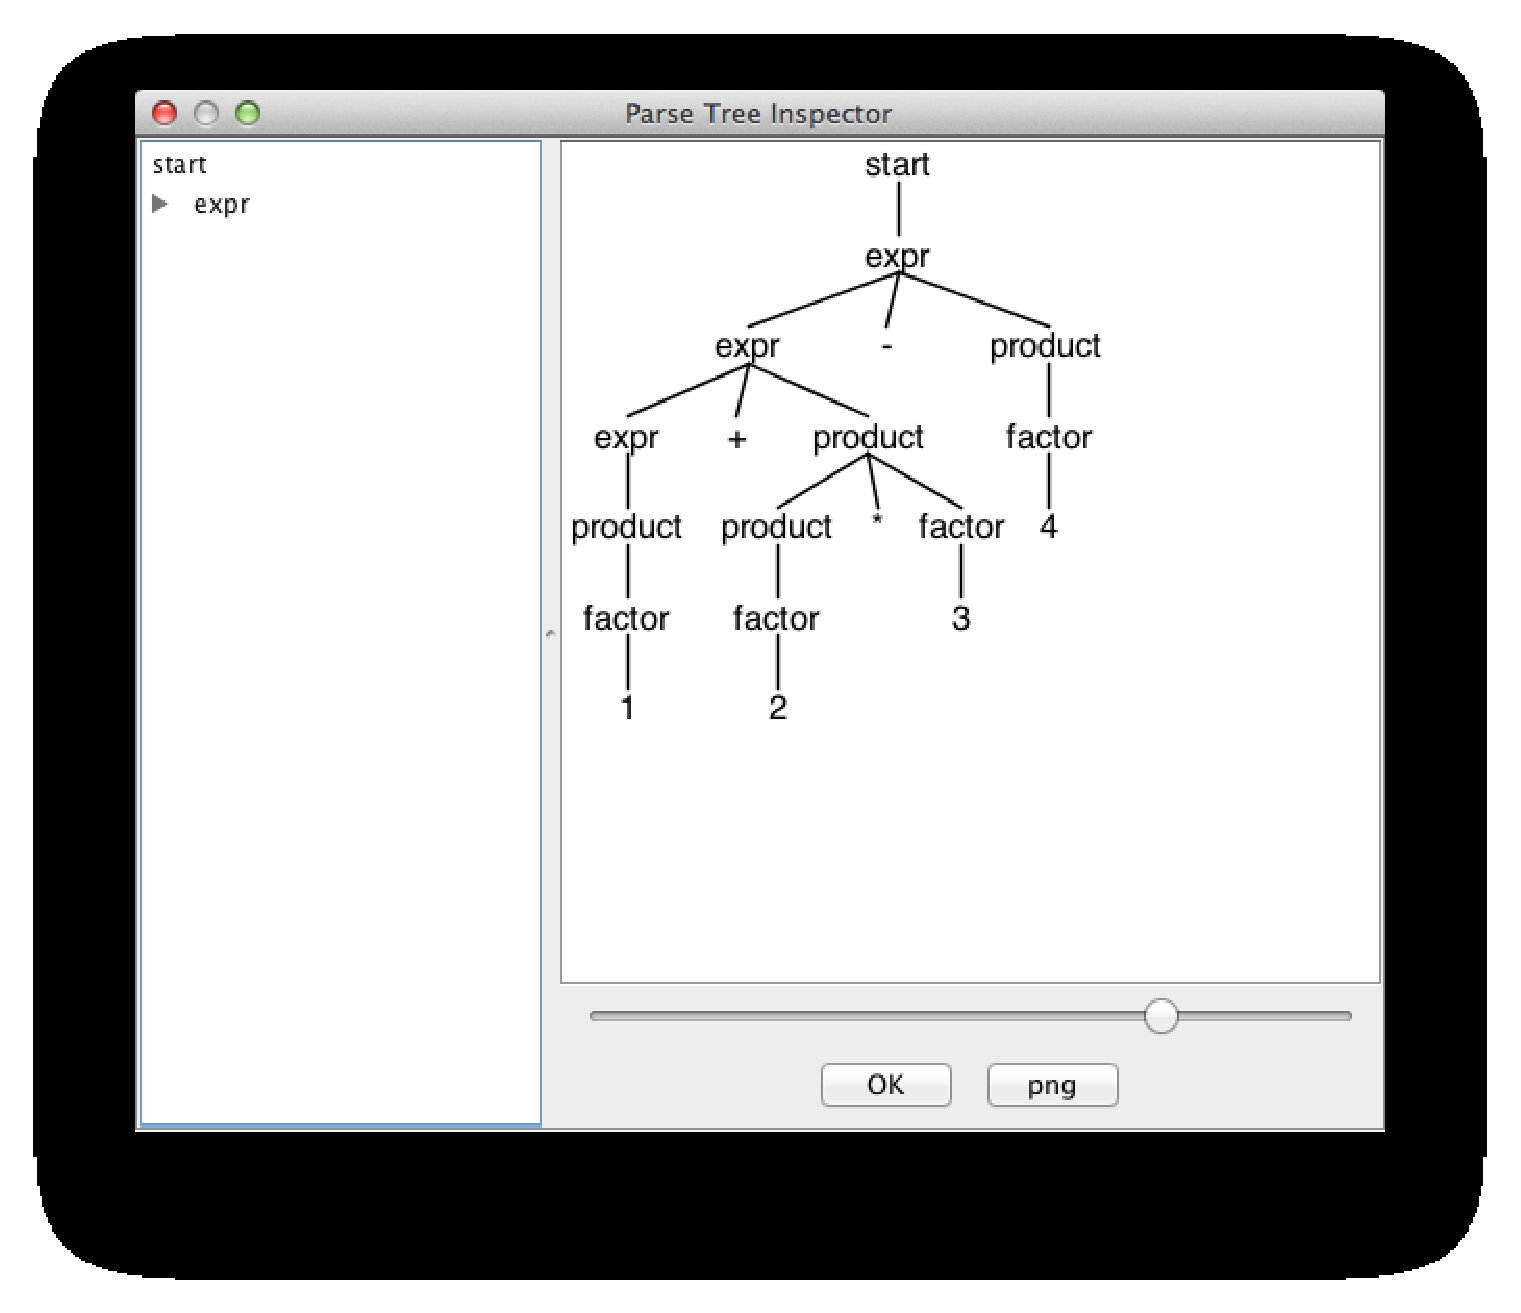
\epsfig{file=Abbildungen/expr.eps, scale=0.7}
   \caption{Syntax-Baum, der beim Parsen des Strings ``\texttt{1+2*3}'' erzeugt wird.}
  \label{fig:expr.eps}
\end{figure}



\section{Ein Parser zur Auswertung arithmetischer Ausdr\"ucke}
Das letzte Beispiel ist noch nicht sehr spektakul\"ar, weil die vom Parser erkannten
Ausdr\"ucke nicht ausgewertet werden.  Wir pr\"asentieren jetzt ein komplexeres Beispiel, bei
dem arithmetische Ausdr\"ucke ausgewertet und die erhaltenen Ergebnisse in Variablen
gespeichert werden k\"onnen.  Wir gehen dabei in zwei Schritten vor und pr\"asentieren
zun\"achst eine reine Grammatik in \textsc{Antlr}-Notation.  Anschlie{\ss}end erweitern wir diese
mit Aktionen, in denen die Ausdr\"ucke ausgewertet werden k\"onnen.
Abbildung \ref{fig:Program.g4} zeigt diese Grammatik.  Gegen\"uber der vorher gezeigten
Grammatik f\"ur arithmetische Ausdr\"ucke gibt es die folgenden \"Anderungen:

\begin{figure}[!ht]
\centering
\begin{Verbatim}[ frame         = lines, 
                  framesep      = 0.3cm, 
                  labelposition = bottomline,
                  numbers       = left,
                  numbersep     = -0.2cm,
                  xleftmargin   = 0.8cm,
                  xrightmargin  = 0.8cm,
                ]
    grammar Program;
    
    program : stmnt+ ;
    
    stmnt   : ID ':=' expr ';'
            | expr ';'
            ;    
    
    expr    : expr ('+'|'-') product
            | product
            ;
    
    product : product ('*'|'/') factor
            | factor
            ;
    
    factor  : '(' expr ')'
            | ID
            | INT
            ;
    
    ID : [a-zA-Z][a-zA-Z0-9]*;
    INT: '0'|[1-9][0-9]*;
    WS : [ \v\t\n\r] -> skip; 
\end{Verbatim}
\vspace*{-0.3cm}
\caption{Eine Grammatik f\"ur die Auswertung von Ausdr\"ucken.}
\label{fig:Program.g4}
\end{figure}


\begin{enumerate}
\item Das Start-Symbol ist jetzt \texttt{program}.  Es steht f\"ur eine Liste
      von Zuweisungen der folgenden Form:
      \\[0.2cm]
      \hspace*{1.3cm}
      $\textsl{var} \;\mathtt{:=}\; \textsl{expr}\mathtt{;}$
      \\[0.2cm]
      Hier ist \texttt{var} der Name einer Variablen und \textsl{expr} ist ein
      arithmetischer Ausdruck.
\item \texttt{stmnt} bezeichnet eine Zuweisung oder einen einzelnen Ausdruck.
\item Wir haben die Regeln f\"ur die syntaktischen Variablen \textsl{expr} und \textsl{product}
      vereinfacht, indem wir jeweils die beiden Operatoren ``\texttt{+}'' und ``\texttt{-}'' bzw.
      \squoted{*} und \squoted{/} zusammengefasst haben.
      Da \textsc{Antlr} \textsc{Ebnf}-Grammatiken unterst\"utzt, k\"onnen wir f\"ur \textsl{expr}
      beispielsweise die Regel
      \\[0.2cm]
      \hspace*{1.3cm}
      \texttt{expr : expr ('+'|'-') product | product ;}
      \\[0.2cm]
      verwenden.  Die Grammatik-Regel f\"ur \textsl{product} haben wir in \"ahnlicher Weise
      ge\"andert.
\item Das Terminal \texttt{ID} bezeichnet den Namen einer Variablen.  Ein solcher Name
      besteht aus einer beliebigen Folge von Buchstaben und Ziffern, die mit einem Buchstaben 
      beginnen muss.
\end{enumerate}
Mit diesem Parser k\"onnen wir jetzt zum Beispiel die folgende Eingabe parsen:
\begin{verbatim}
    x = 2 * 3; y = 4 * 5; z = x * x + y * y; 
    z / 3;
\end{verbatim}
Wir wollen nun einen ganz einfachen Interpreter entwickeln, der eine Folge von solchen
Zuweisungen auswertet und die bei der Auswertung berechneten Zwischen-Ergebnisse
in Variablen abspeichert, auf die in folgenden Ausdr\"ucken Bezug genommen werden kann.
Weiterhin soll jeder Ausdruck, der keiner Variablen zugewiesen wird, ausgewertet und
ausgegeben werden.  Abbildung \ref{fig:Program.g4-2} zeigt die Realisierung eines solchen
Interpreters mit \textsc{Antlr}.

\begin{figure}[!ht]
\centering
\begin{Verbatim}[ frame         = lines, 
                  framesep      = 0.3cm, 
                  labelposition = bottomline,
                  numbers       = left,
                  numbersep     = -0.2cm,
                  xleftmargin   = 0.3cm,
                  xrightmargin  = 0.3cm,
                ]
    grammar Program;
     
    @header {
        import java.util.TreeMap;
    }
    
    @members {
        TreeMap<String, Integer> varTable = new TreeMap<String, Integer>();
    }
    
    program : stmnt+ ;
    
    stmnt : ID ':=' expr ';' { varTable.put($ID.text, $expr.result); }
          |         expr ';' { System.out.println($expr.result);     }
          ;    
    
    expr returns [int result]
        : e = expr { $result = $e.result; }
          (   '+' p = product { $result += $p.result; }
            | '-' p = product { $result -= $p.result; }
          )
        | p = product { $result = $p.result; }
        ;
    
    product returns [int result]
        : p = product { $result = $p.result; }
          (
              '*' f = factor { $result *= $f.result; }
            | '/' f = factor { $result /= $f.result; }
          )
        | f = factor { $result = $f.result; }
        ;
    
    factor returns [int result]
        : '(' expr ')' { $result = $expr.result;           }
        | ID           { $result = varTable.get($ID.text); }
        | INT          { $result = new Integer($INT.text); }
        ;
    
    ID : [a-zA-Z][a-zA-Z0-9]*;
    INT: '0'|[1-9][0-9]*;
    WS : [ \v\t\n\r] -> skip; 
\end{Verbatim} 
%\$
\vspace*{-0.3cm}
\caption{Ein Interpreter zur Auswertung von Ausdr\"ucken.}
\label{fig:Program.g4-2}
\end{figure}

\begin{enumerate}
\item Da wir die Werte der einzelnen Variablen in einer Tabelle abspeichern m\"ussen,
      importieren wir in den Zeilen 3 -- 5 die Klasse \texttt{java.util.TreeMap}, denn
      diese Klasse implementiert Tabellen effizient als bin\"are B\"aume.

      Allgemein setzt \textsc{Antlr} all den Code, der durch das Schl\"usselwort
      ``\texttt{@header}'' spezifiert wird, an den Anfang der erstellten Parser-Datei.
\item In den Zeilen 7 -- 9 definieren wir zus\"atzliche Member-Variablen f\"ur die erzeugte
      Klasse \texttt{ProgramParser}.  In unserem Fall definieren wir hier die Tabelle, die
      sp\"ater die Werte der Variablen enth\"alt, als Abbildung, die Strings ganze Zahlen zuordnet.

      Allgemein setzt \textsc{Antlr} all den Code, der durch das Schl\"usselwort
      ``\texttt{@members}'' spezifiert wird, an den Anfang der erstellten Parser-Klasse.
      Dieses Feature kann sowohl zur Definition von zus\"atzlichen Klassen-Variablen als auch
      von Methoden verwendet werden.
      
      Wir reichern nun die Grammatik-Regeln mit Aktionen an, die durchgef\"uhrt werden, wenn
      der Parser die entsprechende Grammatik-Regel anwendet.  Die Aktionen werden von der
      eigentlichen Grammatik-Regel, f\"ur die sie angewendet werden sollen, dadurch
      abgesetzt, dass sie in den geschweiften Klammern ``\texttt{\{}'' und ``\texttt{\}}''
      eingefasst werden.
\item Wird vom Parser in Zeile 13 eine Zuweisung der Form $\textsl{var} \;\mathtt{:=}\; \textsl{expr}$
      erkannt,  
      so soll der Wert des Ausdrucks \textsl{expr} berechnet und das Ergebnis in der
      Tabelle \texttt{varTable} unter dem Namen \textsl{var} eingetragen werden.
      In der Grammatik-Regel
      \\[0.2cm]
      \hspace*{1.3cm}
      \textsl{stmnt} $\rightarrow$ \texttt{ID} ':=' \textsl{expr} ';'
      \\[0.2cm]
      haben wir einerseits das Token \texttt{ID}, auf dessen Namen wir mit \texttt{\symbol{36}ID.text}
      zugreifen k\"onnen, andererseits haben wir die syntaktische Variable \textsl{expr}.
      Wir werden sp\"ater dieser syntaktischen Variable die \textsl{Java}-Variable
      \texttt{result} als Ergebnis-Variable zuordnen, die den zugeh\"origen Wert enth\"alt.  
      Dann k\"onnen wir mit
      \texttt{\symbol{36}expr.result} auf diesen Wert zugreifen.

      In Zeile 14 haben wir einen einzelnen arithmetischen Ausdruck, den wir auswerten und ausgeben.
\item In Zeile 17 definieren wir mit der Zeile
      \\[0.2cm]
      \hspace*{1.3cm}
      \texttt{expr returns [int result]}
      \\[0.2cm]
      dass die Methode, die eine \textsl{expr} parst, als Ergebnis ein \texttt{int} zur\"uck
      gibt und dass dieses in der Variable mit dem Namen \texttt{result} abgespeichert wird.
\item In der Grammatik-Regel
      \\[0.2cm]
      \hspace*{1.3cm}
      \texttt{expr : expr ('+'|'-') product | product ;}
      \\[0.2cm]
      haben wir in Zeile 18 -- 20 den verschiedenen Auftreten der syntaktischen Variablen
      \texttt{expr} und \texttt{product} die Namen $e$ und $p$ zugeordnet, auf die wir dann in den
      Aktionen zugreifen k\"onnen.  In den Aktionen muss diesen Variablen allerdings ein Dollar-Zeichen
      vorgestellt werden.

      Die Aktionen selber bestehen nun darin, dass wir der Variablen \texttt{result}
      das Ergebnis der jeweiligen Berechnung zuweisen.
\item In den Zeilen 36 und 37 greifen wir auf die Strings, die den Token
      \texttt{ID} und \texttt{INT} entsprechen, mit Hilfe der f\"ur Token vordefinierten
      Variable \texttt{text} zur\"uck.  Beachten Sie, dass wir in Zeile 36 den Wert, der zu einer
      Variablen in der Tabelle \texttt{varTable} gespeichert ist, auslesen und als Ergebnis zur\"uck
      geben. 
\end{enumerate}

\section{Erzeugung abstrakter Syntax-B\"aume}
Bei der Auswertung arithmetischer Ausdr\"ucke im letzten Abschnitt hatten wir Gl\"uck
und konnten das Ergebnis eines Ausdrucks unmittelbar mit Hilfe von semantischen Aktionen
berechnen.  Bei komplexeren Problemen ist es in der Regel erforderlich, zun\"achst einen
abstrakten Syntax-Baum zu erzeugen.  Die eigentliche Berechnung findet dann erst nach dem
Parsen auf dem Syntax-Baum statt.  Wir wollen dieses Verfahren an einem Beispiel
demonstrieren.  Bei dem Beispiel geht es wieder um die symbolische Differentiation
arithmetischer Ausdr\"ucke.  Ist beispielsweise der arithmetische Ausdruck 
\[ x \cdot \ln(x) \]
gegeben, so findet sich f\"ur die Ableitung dieses Ausdrucks nach der Variable $x$ mit Hilfe
der Produkt-Regel das
Ergebnis 
\[ 1 \cdot \ln(x) + x \cdot \frac{1}{x}. \]  
Da die arithmetischen Ausdr\"ucke nun
zus\"atzlich zu den Operatoren, welche die vier Grundrechenarten beschreiben, auch noch 
Funktionszeichen f\"ur die Exponential-Funktion und den nat\"urlichen Logarithmus enthalten
sollen, m\"ussen wir die Grammatik aus dem letzten Abschnitt erweitern.
Abbildung \ref{fig:Expr-exp-ln} zeigt die entsprechend erweiterte EBNF-Grammatik.

\begin{figure}[htbp]
  \begin{center}    
  \framebox{
  \framebox{
  \begin{minipage}[t]{9cm}

  \begin{eqnarray*}
  \textsl{expr}   & \rightarrow & \;\textsl{expr}\;\;(\quoted{+}|\quoted{-})  \;\; \textsl{product}  \\
                  & \mid        & \textsl{product}                                 \\[0.2cm]
  \textsl{product} & \rightarrow & \;\textsl{product}\;\;\;\;(\quoted{*}|\quoted{/}) \;\; \textsl{factor} \\
                  & \mid        & \textsl{factor}  \\[0.2cm]
  \textsl{factor} & \rightarrow & \quoted{(} \textsl{expr} \quoted{)}              \\
                  & \mid        & \quoted{exp} \quoted{(} \textsl{expr} \quoted{)} \\
                  & \mid        & \quoted{log} \quoted{(} \textsl{expr} \quoted{)} \\
                  & \mid        & \;\textsc{Variable}                              \\
                  & \mid        & \;\textsc{Number} 
  \end{eqnarray*}
  \vspace*{-0.5cm}

  \end{minipage}}}
  \end{center}
  \caption{EBNF-Grammatik f\"ur arithmetische Ausdr\"ucke mit Exponential-Funktion und Logarithmus.}
  \label{fig:Expr-exp-ln}
\end{figure}

\subsection{Implementierung des Parsers}
Abbildung \ref{fig:grammatik.g} zeigt die \textsc{Antlr}-Implementierung der Grammatik
aus Abbildung \ref{fig:Expr-exp-ln}.  

\begin{figure}[!ht]
\centering
\begin{Verbatim}[ frame         = lines, 
                  framesep      = 0.3cm, 
                  labelposition = bottomline,
                  numbers       = left,
                  numbersep     = -0.2cm,
                  xleftmargin   = 0.0cm,
                  xrightmargin  = 0.0cm,
                ]
    grammar Expr;
    
    expr returns [Expr result]
        : e = expr '+' p = product { $result = new Sum(       $e.result, $p.result); }
        | e = expr '-' p = product { $result = new Difference($e.result, $p.result); }
        | p = product              { $result = $p.result; }    
        ;
    
    product returns [Expr result]
        : p = product '*' f = factor { $result = new Product( $p.result, $f.result); }
        | p = product '/' f = factor { $result = new Quotient($p.result, $f.result); }
        | f = factor                 { $result = $f.result; }
        ;
    
    factor returns [Expr result]
        : '(' expr ')'       { $result = $expr.result;                  }
        | 'exp' '(' expr ')' { $result = new Exponential($expr.result); }
        | 'log' '(' expr ')' { $result = new Logarithm(  $expr.result); }
        | VAR                { $result = new Variable($VAR.text);       }
        | NUM                { $result = new Number($NUM.text);         }
        ;
    
    VAR : [a-zA-Z][a-zA-Z0-9]*;
    NUM : '0'|[1-9][0-9]*;
    WS  : [ \v\t\n\r] -> skip; 
\end{Verbatim}
\vspace*{-0.3cm}
\caption{Die \textsc{Antlr}-Spezifikation der Grammatik.}
\label{fig:grammatik.g}
\end{figure}

\begin{enumerate}
\item In Zeile 3 deklarieren wir durch ``\texttt{returns [Expr result]}'',
      dass beim Erkennen einer \textsl{expr} nun ein Objekt der Klasse \texttt{Expr}
      zur\"uck gegeben werden soll und dass dieses Objekt \"uber den Namen
      \texttt{result} angesprochen werden kann.  Die Klasse \texttt{Expr} ist hier eine abstrakte
      Klasse, von der wir die Klassen
      \begin{enumerate}
      \item \texttt{Sum} (zur Darstellung von Termen der Form $s + t$),
      \item \texttt{Difference} (zur Darstellung von Termen der Form $s - t$),
      \item \texttt{Product} (zur Darstellung von Termen der Form $s * t$),
      \item \texttt{Quotient} (zur Darstellung von Termen der Form $s / t$),
      \item \texttt{Exponential} (zur Darstellung von Termen der Form $\textsl{exp}(s)$),
      \item \texttt{Logarithm} (zur Darstellung von Termen der Form $\textsl{ln}(s)$),
      \item \texttt{Number} (zur Darstellung von Zahlen) und
      \item \texttt{Variable} (zur Darstellung von Variablen)
      \end{enumerate}
      ableiten.  Die Klasse \texttt{Expr} besitzt nur die abstrakte Methode 
      \\[0.2cm]
      \hspace*{1.3cm}
      \texttt{public abstract Expr diff(String x);}
      \\[0.2cm]
      die dazu benutzt wird, einen arithmetischen Ausdruck nach einer gegebenen Variablen
      abzuleiten.  Die von \texttt{Expr} abgeleiteten Klassen sind alle nach dem gleichen Muster
      aufgebaut.  Beispielhaft zeigt Abbildung \ref{fig:Product.java} auf Seite \pageref{fig:Product.java}
        die Implementierung der Klasse 
      \texttt{Product}.
      \begin{enumerate}
      \item Die Klasse beinhaltet die beiden Member-Variablen \texttt{mLhs} und \texttt{mRhs}.
            Ein Objekt der Klasse \texttt{Product} wird als das Produkt
            \\[0.2cm]
            \hspace*{1.3cm}
            $\mathtt{mLhs} * \mathtt{mRhs}$
            \\[0.2cm]
            interpretiert.
      \item Zus\"atzlich gibt es eine Implementierung der Methode \texttt{diff}, in der die
            Produkt-Regel umgesetzt wird.
      \item Zur Ausgabe ist weiterhin eine \texttt{toString}-Methode vorhanden.
      \end{enumerate}

\begin{figure}[!ht]
\centering
\begin{Verbatim}[ frame         = lines, 
                  framesep      = 0.3cm, 
                  firstnumber   = 1,
                  labelposition = bottomline,
                  numbers       = left,
                  numbersep     = -0.2cm,
                  xleftmargin   = 0.0cm,
                  xrightmargin  = 0.0cm,
                ]
    public class Product extends Expr {
        private Expr mLhs;
        private Expr mRhs;
    
        public Product(Expr lhs, Expr rhs) {
            mLhs = lhs;
            mRhs = rhs;
        }
        public Expr diff(String x) {
            return new Sum(new Product(mLhs.diff(x), mRhs), new Product(mLhs, mRhs.diff(x)));
        }
        public String toString() {
            return mLhs.toString() + " * " + mRhs.toString();
        }
    }
\end{Verbatim}
\vspace*{-0.3cm}
\caption{Die Klasse \texttt{Product} zur Darstellung von Produkten.}
\label{fig:Product.java}
\end{figure}

      
      
\item In Zeile 4 haben wir zun\"achst ein Produkt erkannt, dass wir unter der Variable
      $p$ abspeichern.  Anschlie{\ss}end weisen wir der Variable \texttt{result} dieses
      Produkt zu.  Falls nun sp\"ater noch ein ``\texttt{+}''-- oder ``\texttt{-}''
      Zeichen gefolgt von einem weiteren Ausdruck gelesen wird, so bauen wir aus dem neu
      gelesenen Ausdruck und dem alten Wert von \texttt{result} den neuen Wert von
      \texttt{result}.  Dies kann mehrmals passieren, da dieser Teil der Grammatik-Regel
      in $( \cdots )*$ eingeschlossen ist.
      
      Beispielsweise wird ein Ausdruck der Form
      \\[0.2cm]
      \hspace*{1.3cm}
      $p_1 + p_2 + p_3$
      \\[0.2cm]
      \"ubersetzt in ein Java-Objekt der Form
      \\[0.2cm]
      \hspace*{1.3cm}
      $\texttt{new\ Sum}(\texttt{new\ Sum}(p_1, p_2), p_3))$.       
\item Die weiteren Grammatik-Regeln erzeugen in analoger Weise \textsl{Java}-Objekte.
\end{enumerate}

Zum Abschluss zeigt Abbildung \ref{fig:Differentiate.java} noch die Einbindung des Parsers.
Gegen\"uber dem in Abbildung \ref{fig:ParseExpr.java} gezeigten Treiber gibt es nur einen
wesentlichen Unterschied: In Zeile 20 wird nun ein Objekt der Klasse \texttt{Expr} erzeugt.
Beachten Sie, dass der Aufruf
\\[0.2cm]
\hspace*{1.3cm}
\texttt{parser.expr()}
\\[0.2cm]
zun\"achst ein Objekt der Klasse \texttt{ExprParser.ExprContext} erzeugt.  Bei dieser Klasse handelt
es sich um eine innere Klasse der Klasse \texttt{ExprParser}.  Die innere Klasse
\texttt{ExprContext} enth\"alt nun eine Member-Variable mit dem Namen \texttt{result}, in der die
eigentliche \texttt{Expr} gespeichert ist.  
F\"ur dieses Objekt rufen wir dann in Zeile 21 die Methode $\textsl{diff}()$ auf, welche die
symbolische Ableitung berechnet.


\begin{figure}[!ht]
\centering
\begin{Verbatim}[ frame         = lines, 
                  framesep      = 0.3cm, 
                  labelposition = bottomline,
                  numbers       = left,
                  numbersep     = -0.2cm,
                  xleftmargin   = 0.8cm,
                  xrightmargin  = 0.8cm,
                ]
    import org.antlr.v4.runtime.*;
    import java.io.FileInputStream;
    import java.io.InputStream;
    
    public class Differentiate {
    
        public static void main(String[] args) throws Exception {
            String inputFile = null; 
            if (args.length > 0) { 
    	    inputFile = args[0];
    	}
            InputStream is = System.in;
            if (inputFile != null) {
    	    is = new FileInputStream(inputFile);
    	}
            ANTLRInputStream  input  = new ANTLRInputStream(is);
            ExprLexer         lexer  = new ExprLexer(input);
            CommonTokenStream ts     = new CommonTokenStream(lexer);
            ExprParser        parser = new ExprParser(ts);
            Expr expr = parser.expr().result;
            Expr diff = expr.diff("x");
            System.out.println("d (" + expr + ")/dx = " + diff);
        }
    }
\end{Verbatim}
\vspace*{-0.3cm}
\caption{Ein Treiber f\"ur den Parser.}
\label{fig:Differentiate.java}
\end{figure}
\pagebreak


\exerciseEng
The \href{https://github.com/karlstroetmann/Formal-Languages}{github directory} associated with this lecture
contains the file
\\[0.2cm]
\hspace*{1.3cm}
\href{https://github.com/karlstroetmann/Formal-Languages/tree/master/Exercises/Grammar2HTML-Antlr/c-grammar.g}{
\texttt{Exercises/Grammar2HTML-Antlr/c-grammar.g}}
\\[0.2cm]
that specifies the syntax of the programming language 
\href{https://en.wikipedia.org/wiki/C_(programming_language)}{\texttt{C}}.

\begin{enumerate}[(a)]
\item Your first task is specify the syntax used to denote the grammar rules given in the file
      \texttt{c-grammar.g}.  Of course, in order to specify this syntax you should use a
      context-free grammar. 
\item Next, you should develop a parser that is capable of reading the file \texttt{c-grammar.g}
      and that, furthermore, can convert this grammar into \textsc{Html}. 
      This parser should be developed using the tool \textsc{Antlr}.
\end{enumerate}

\remarkEng
\begin{enumerate}
\item The directory 
      \\[0.2cm]
      \hspace*{1.3cm}
      \href{https://github.com/karlstroetmann/Formal-Languages/tree/master/Exercises/Grammar2HTML/}{\texttt{Exercises/Grammar2HTML}}
      \\[0.2cm]
      contains several classes that represent various nodes of an abstract syntax tree corresponding to a
      given grammar.  The given classes already contain an implementation of the method $\texttt{toString}()$. This method 
      converts a node of the abstract syntax tree into an \textsc{Html} string.
\item \textsc{Antlr} provides a negation operator that is written as ``\texttt{\symbol{126}}''.
      Using the negation operator comes in handy when recognizing \emph{literal tokens},  
      i.e.~tokens that represent either keywords or operators of the language \texttt{C}.  In the
      file \texttt{c-grammar.g}, literal tokens are enclosed in single quotes.
\item For obscure historical reasons, \textsc{Antlr} treats the string ``\texttt{rule}'' as a 
      keyword.  Therefore, it is not possible to have a syntactical variable that is called
      ``\texttt{rule}''. 
\end{enumerate}



%%% Local Variables: 
%%% mode: latex
%%% TeX-master: "formal-languages"
%%% End: 
